\documentclass{report}

\usepackage{amsmath,amsfonts,amsthm,amssymb,mathtools}

\usepackage[most]{tcolorbox}

\usepackage{blindtext} %Lorem Ipsum

\usepackage{titlesec} %Custom Section Titles

\usepackage{pgfplots}
\usetikzlibrary{patterns}

\pgfplotsset{compat=1.18}
\titleformat
{\chapter} % command
[display] % shape
{\bfseries\Large\itshape} % format
{Part\ \thechapter} % label
{0.5ex} % sep
{
    \rule{\textwidth}{1pt}
    \vspace{1ex}
    \centering
} % before-code
[
\vspace{-1.5ex}%
\rule{\textwidth}{0.3pt}
] % after-code
\titlespacing*{\chapter}{0pt}{-50pt}{8pt}
%Theorem Boxes
%
\newtcolorbox{thm}[2][]{
  enhanced jigsaw, % better frame drawing
  sharp corners, % No rounded corners
  boxrule=1pt, % thin frame
  fonttitle={\large\bfseries},
  coltitle={white},  % white colour for title
  colframe = red!30, %red border
  colback = red!5, %cyan background
  title=Theorem: {#2} ,  % Fixed title
  #1
}

\newtcolorbox{cor}[2][]{
  enhanced jigsaw, % better frame drawing
  sharp corners, % No rounded corners
  borderline west={2pt}{0pt}{pink}, % straight vertical line at the left edge
  boxrule=0pt, % thin frame
  fonttitle={\large\bfseries},
  coltitle={black},  % white colour for title
  colback = pink!5, %cyan background
  title=Corollary: {#2} \\,  % Fixed title
  attach title to upper,
  #1
}

\newtcolorbox{lem}[2][]{
  enhanced jigsaw, % better frame drawing
  sharp corners, % No rounded corners
  borderline west={2pt}{0pt}{violet!35}, % straight vertical line at the left edge
  boxrule=0pt, % thin frame
  fonttitle={\large\bfseries},
  coltitle={black},  % white colour for title
  colframe = green!25, %red border
  colback = violet!2, %cyan background
  title=Lemma: {#2} \\,  % Fixed title
  attach title to upper,
  #1
}

\newtcolorbox{dfn}[2][]{%
  enhanced jigsaw, % better frame drawing
  sharp corners, % No rounded corners
  boxrule=1pt,  % thin frame
  fonttitle={\large\bfseries},
  coltitle={white},  % white colour for title
  colframe = blue!30, %blue border
  colback = blue!5, %cyan background
  title={Definition: {#2}\ },  % Fixed title
  #1
}

\newtcolorbox{ex}[2][]{%
  enhanced jigsaw, % better frame drawing
  sharp corners, % No rounded corners
  boxrule=1pt,  % thin frame
  fonttitle={\large\bfseries},
  coltitle={black},  % white colour for title
  colframe = cyan!20, %cyan border
  colback = cyan!5, %cyan background
  title={Example: {#2} \ },  % Fixed title
  attach title to upper,
  #1
}

\newtcolorbox{note}[1][]{%
  enhanced jigsaw, % better frame drawing
  borderline west={2pt}{0pt}{red}, % straight vertical line at the left edge
  sharp corners, % No rounded corners
  boxrule=0pt, % no real frame,
  fonttitle={\large\bfseries},
  coltitle={black},  % Black colour for title
  title={Note: \ },  % Fixed title
  attach title to upper, % Move the title into the box
  #1
}

\newtcolorbox{question}[2][]{%
  enhanced jigsaw, % better frame drawing
  borderline west={2pt}{0pt}{green}, % straight vertical line at the left edge
  sharp corners, % No rounded corners
  boxrule=0pt, % no real frame,
  fonttitle={\large\bfseries},
  coltitle={black},  % Black colour for title
  colback={green!5},
  title={Question {#2}: \ },  % Fixed title
  attach title to upper, % Move the title into the box
  #1
}

%Change QED Symbol%
\renewcommand\qedsymbol{$\blacksquare$}

\author{\huge Ryan Arif\\ \normalsize }
\title{\huge Graduate Mathematical Analysis\\Notes\\\normalsize Instructor: Dr. Barbra Shipman, University of Texas at Arlington}
\date{Fall 2025}

\begin{document}
\maketitle
\tableofcontents

\pagebreak
\section*{Preface}
In this course, two textbooks will be used as references:
\begin{itemize}
    \item \textbf{Mathematical Analysis} by Tom M. Apostol,
    \item \textbf{Understanding Analysis} by Stephen Abbott.
\end{itemize}

Any references to sections or exercises will be from these books unless otherwise specified.
Most of the content will be based on Abbott, but Apostol has some topics Abbott lacks.

These are mostly lectures notes \& homeworks and solutions.

Also, note, I'm an undergraduate student. I like to think I'm smart, but I make a lot of mistakes.

If you catch one, let me know. You can make it fun by proving me wrong, I love learning.

\begin{note}
    These notes were written in VSCode. Unfortunately, AI is like, built into VSCode now.

    Fortunately, the AI is very handy for making the plots and pictures you'll see in the notes.

    Sometimes, the AI makes suggestions for proofs and content. I don't accept these suggestions and edits.

    Also, these notes are a compilation of my work. I've already done the work on pen and paper, I'm just typing it up here.
\end{note}
\chapter{The Real Number System \& Set Theory}
\begin{center}
Book References:

Apostol: 1.1 – 1.19, 2.1 – 2.15

Abbott: 1.1 – 1.7
\end{center}

In this section, we will cover:
\begin{itemize}
    \item The Real Number System
    \item Bounds
    \item Functions
    \item Set Theory
    \item Cardinality
\end{itemize}

\section{Topic 1}
This is the content for Topic 1.
\begin{thm}{Sample Theorem}
This is a sample theorem in Topic 1.
\end{thm}

\begin{proof}
    Yes.
\end{proof}

This concludes part 1 of Mathematical Analysis.

\setcounter{chapter}{5}
\chapter{Integration \& The Fundamental Theorem of Calculus}
\begin{center}
Book References:

Abbott: Chapter 7
\end{center}

In this section, we will cover:
\begin{itemize}
    \item The Reimann Integral
    \item Criteria for Integability
    \item Properties of the Integral
    \item The Fundamental Theorem of Calculus
\end{itemize}

\section{The Reimann Integral}
This is really the regular integral from Calculus! We'll end up making it a bit more rigorous, but it's going to work the way that you'd hope.
First, let's start with a few examples from Calculus class.
\begin{ex}{}
    \begin{center}
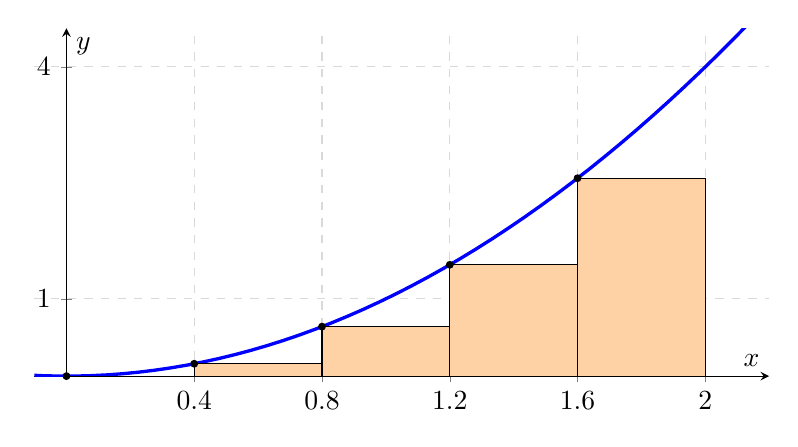
\begin{tikzpicture}
  \begin{axis}[
    width=0.9\textwidth, height=6cm,
    axis lines=middle,
    xlabel={$x$}, ylabel={$y$},
    xmin=-0.1, xmax=2.2, ymin=0, ymax=4.5,
    xtick={0,0.4,0.8,1.2,1.6,2},
    ytick={0,1,4},
    grid=major, grid style={dashed,gray!30},
    samples=200,
  ]
    \addplot [very thick, blue] {x^2};

    \foreach \i in {0,1,2,3,4} {
      \pgfmathsetmacro{\x}{\i*0.4}
      \pgfmathsetmacro{\h}{\x*\x}
      \addplot [draw=black, fill=orange!35] coordinates
        {(\x,0) (\x,{\h}) ({\x+0.4},{\h}) ({\x+0.4},0)} \closedcycle;
    }

    \foreach \i in {0,1,2,3,4} {
      \pgfmathsetmacro{\x}{\i*0.4}
      \pgfmathsetmacro{\h}{\x*\x}
      \addplot[black, mark=*, mark options={scale=0.6}] coordinates {(\x,{\h})};
    }
  \end{axis}
\end{tikzpicture}
\par\smallskip
    \end{center}

Using really basic calculus, we can definitely integrate it. This is a Continuous curve, so it's integrable.
We can use rectangles to compute the Riemann sum of this.

If we had a constant function, the Riemann sum wouldn't be an approximation, but exactly the integral.
\end{ex}

In Analysis, though, we don't require continuity for integrability. Let's examine a fun function.

\begin{ex}{Dirichlet Function}
    \begin{center}
    The Dirichlet function is defined as:
    \[
    D(x) = \begin{cases}
    1 & \text{if } x \in \mathbb{Q} \\
    0 & \text{if } x \notin \mathbb{Q}
    \end{cases}
    \]


    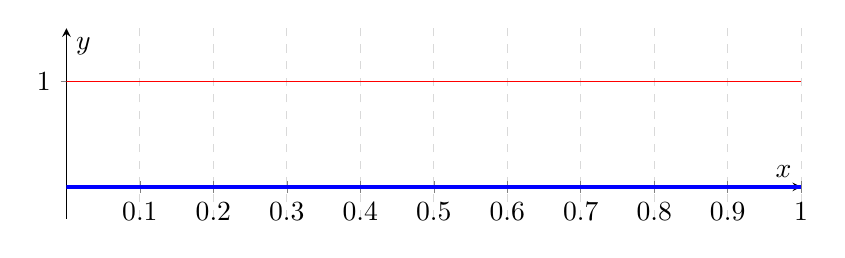
\begin{tikzpicture}
        \begin{axis}[
            width=0.9\textwidth, height=4cm,
            axis lines=middle,
            xlabel={$x$}, ylabel={$y$},
            xmin=0, xmax=1, ymin=-0.3, ymax=1.5,
            ytick={0,1},
            grid=major, grid style={dashed,gray!30},
        ]
            \addplot [ultra thick, blue, domain=0:1] {0};
            \addplot [thin, red, domain=0:1] {1};
        \end{axis}
    \end{tikzpicture}
    \par\smallskip
    \textbf{Figure.} $D(x) = 1$ for $x \in \mathbb{Q}$ (thin red line) and $D(x) = 0$ for $x \notin \mathbb{Q}$ (bold blue line).
    \end{center}
    Let's try integrating it the calculus way.

    We'd have to pick our endpoints, first. Let's have our rectangles start from the left, at 0. Let's pick 5 or so subintervals.
    
    \begin{center}
    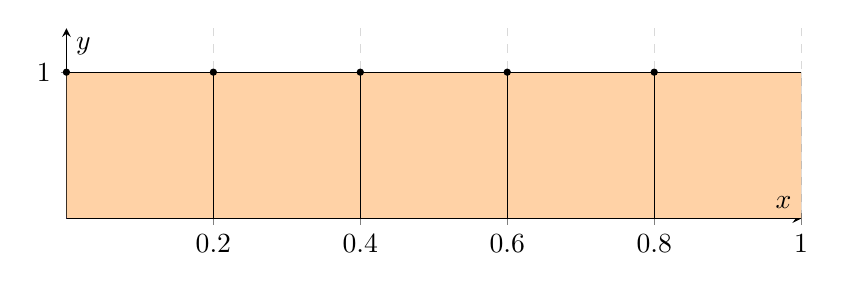
\begin{tikzpicture}
        \begin{axis}[
            width=0.9\textwidth, height=4cm,
            axis lines=middle,
            xlabel={$x$}, ylabel={$y$},
            xmin=0, xmax=1, ymin=0, ymax=1.3,
            xtick={0,0.2,0.4,0.6,0.8,1},
            ytick={0,1},
            grid=major, grid style={dashed,gray!30},
        ]
            % Dirichlet function “graph”
            \addplot[ultra thick, blue, domain=0:1] {0};
            \addplot[thin, red, domain=0:1] {1};

            % Left-endpoint Riemann sum with 5 subintervals
            \foreach \i in {0,...,4} {
                \pgfmathsetmacro{\x}{\i*0.2}
                \addplot[draw=black, fill=orange!35] coordinates
                    {(\x,0) (\x,1) ({\x+0.2},1) ({\x+0.2},0)} \closedcycle;
                \addplot[black, mark=*, mark options={scale=0.55}] coordinates {(\x,1)};
            }
        \end{axis}
    \end{tikzpicture}
    \par\smallskip
    \end{center}

    I mean, clearly, 
    \begin{align}
    \int_{0}^{1}D(x)dx = 1
    \end{align}
    Well, what if we change up the endpoints? It's entirely possible to pick irrationals for our endpoints, which lay on 0.

    So, then, 
    \begin{align}
        \int_{0}^{1}D(x)dx = 0.
    \end{align}
    We clearly have some disagreement here, and have another great example of the failure of Calculus classes.
\end{ex}


The above example is great motivation for us to create a much better definition of an integral.

\section{Criteria for Integrability}

\begin{dfn}{Integability}
Let $f$ be a bounded function on $[a,b]$.
Create a partition $P$ of $[a,b]$ such that
\[ P = \{a = x_0, x_1, x_2, \ldots, x_n = b : x_0 < x_1 < \ldots < x_n\} \]
Which has a handy shorthand, $P = \{a=x_0 < x_1 < \ldots < x_n = b\}$.
Create the upper sum, $U(f,P)$,
\[ U = \sum_{k=1}^{n}M_k \Delta x_k \]
where $M_k = \sup{f(x) : x \in [x_{k-1}, x_k]}$ and $\Delta x_k = x_k - x_{k-1}$.

And the lower sum, $L(f,P)$,
\[ L = \sum_{k=1}^{n}m_k \Delta x_k \]
where $m_k = \inf{f(x) : x \in [x_{k-1}, x_k]}$ and $\Delta x_k = x_k - x_{k-1}$.

Define the upper integral as
\[ \overline{\int_{a}^{b}} f(x) dx = \inf\{U(f,P) : P \text{ is a partition of } [a,b]\} \]

Define the lower integral as
\[ \underline{\int_{a}^{b}} f(x) dx = \sup\{L(f,P) : P \text{ is a partition of } [a,b]\} \]

To say that $f$ is integrable on $[a,b]$ means that $U(f) = L(f)$, and 
\[\int_{a}^{b} f(x) dx = U(f) = L(f) \].

\end{dfn}

Wow, what a mouthful.

Let's talk about this in a slightly different register.

To say that a function is integrable means the lower and upper sums are going to the same number.
That number is the value of the integral.

We may be able to think about this as a convergence (Which we can! We will prove this later!)

\begin{note}
    Notice that this definition doesn't mention continuity, or antiderivatives.

    Calculus class kind of gives you the idea that integration = antidifferentiation, but those are two separate concepts.
    We will make a connection between them later, with FTC, but they are still not the same thing.
\end{note}

Let's do a quick example.

\begin{ex}{Line with Discontinuity}
    Consider the function:
    \[
    f(x) = \begin{cases}
    0 & \text{if } x \neq \frac{1}{2} \\
    1 & \text{if } x = \frac{1}{2}
    \end{cases}
    \]
    on $[0,1]$.

    \begin{center}
    \begin{tikzpicture}
        \begin{axis}[
            width=0.9\textwidth, height=4cm,
            axis lines=middle,
            xlabel={$x$}, ylabel={$y$},
            xmin=-0.05, xmax=1.05, ymin=-0.2, ymax=1.3,
            xtick={0,0.5,1},
            xticklabels={0,$\frac{1}{2}$,1},
            ytick={0,1},
            grid=major, grid style={dashed,gray!30},
        ]
            % The function is 0 everywhere except at x=1/2
            \addplot[ultra thick, blue, domain=0:0.49] {0};
            \addplot[ultra thick, blue, domain=0.51:1] {0};
            
            % Open circle at (0.5, 0) to show discontinuity
            \addplot[blue, mark=o, mark options={scale=1.5, fill=white}] coordinates {(0.5,0)};
            
            % Closed circle at (0.5, 1) to show the value there
            \addplot[blue, mark=*, mark options={scale=1.5}] coordinates {(0.5,1)};
        \end{axis}
    \end{tikzpicture}
    \par\smallskip

    Let's integrate this with our new technique.

    Let's pick a partition, $P = \{0, \frac{1}{2} - \epsilon, \frac{1}{2} + \epsilon, 1\}$ where $\epsilon > 0$.

    So, $U(f,P) = 0 \cdot 0 + | \frac{1}{2} + \epsilon - (\frac{1}{2} - \epsilon)| \cdot 1 + 0 \cdot 0 = 2\epsilon$.

    And, $L(f,P) = 0 \cdot 0 + | \frac{1}{2} + \epsilon - (\frac{1}{2} - \epsilon)| \cdot 0 + 0 \cdot 0 = 0$.

    Of course, $2 \epsilon \neq 0$. But again, if we think about this as a limit, we can say $\epsilon$ is arbitrarily small, so this goes to $0$.
    \end{center}
\end{ex}

Let's build upon this example with a theorem.

\begin{thm}{$\epsilon$-Criterion for Integrability}
    Let $f$ be bounded on $[a,b]$.

    Then, $\int_{a}^{b} f(x) dx$ exists $\iff$ for all $\epsilon > 0$, there is a partition $P_{\epsilon}$ such that $U(f,P_\epsilon) - L(f,P_\epsilon) < \epsilon$.
\end{thm}

This wasn't proven in class, so I'm not going to try to prove it here.

It's not difficult to prove, it relies heavily on the definitions.

Another integration theorem, it's very handy. It's not something we'll prove.

\begin{thm}{Lebesgue's Theorem}
    Suppose $f$ is bounded on $[a,b]$.

    Then, $\int_{a}^{b} f(x) dx$ exists if and only if the set of points where $f$ is discontinuous has measure zero.

\end{thm}

What's measure zero, though? Not very helpful.

We can think about it like, if we remove all of the discontinuities, we still have basically the same set.

If we consider the above example, the function with the whole that goes up at a single point, by plucking out that one point we don't really change anything.

Here's a better definition, though, for measure zero.

\begin{dfn}{Measure Zero}
    To say that $A \subseteq \mathbb{R}$ has measure zero means that

    For all $\epsilon > 0$, there exists a countable collection of open intervals,

    \[ \{O_i : i \in I\} \]

    Such that,

    \begin{enumerate}
        \item $A \subseteq \bigcup_{i \in I} O_i$,
        \item $\sum_{i \in I} \text{length}(O_i) < \epsilon$.
    \end{enumerate}
\end{dfn}

So, if we can remove the discontinuities, and those discontinuities have a 1:1 correspondence with the naturals, we're good to integrate.

\section{The Fundamental Theorem of Calculus}
This is probably my favorite section of any analysis class.

The fundamental theorem of calculus connects the two different topics of integration, differentiation, and anti-differentiation.

Recall our definition of the integral. It has absolutely nothing to do with antiderivatives. Yet, Calculus Class seems to give us the idea that the two are connected, and that the definition of integral uses the antiderivative.

I seriously cannot stress enough how wrong that is. Calculus Class needs to do better at making the two distinct. Renaming the antiderivative to the "indefinite integral" was a huge mistake, and I will personally never use it.

Okay, without any further ado, here's the FTC.

\begin{thm}{Fundamental Theorem of Calculus Part 1}
    Suppose $f$ is integrable on $[a,b]$, and that $F'(x) = f(x)$ on $[a,b]$.

    Then, 
    \[
    \int_{a}^{b} f(x) \, dx = F(b) - F(a).
    \]
\end{thm}
The proof for this isn't the craziest thing in the world.

Dr. Shipman specifically says, this is "a good one to know...". It could absolutely be on \textbf{any} exam.

\begin{proof}
    Let $P$ be a partition of $[a,b]$.

    On each subinterval, $[x_{k-1}, x_k]$, apply the Mean Value Theorem to $F$:

    So,
    \begin{align}
    \exists c_k \in (x_{k-1}, x_k) \text{ such that } \frac{F(x_k) - F(x_{k-1})}{x_k - x_{k-1}} = F'(c_k) = f(c_k).
    \end{align}

    Rearrange this, we have:
    \[ F(x_k) - F(x_{k-1}) = f(c_k)(x_k - x_{k-1}) = f(c_k) \Delta x_k. \]
    Notice that for all $k$, $m_k \leq f(c_k) \leq M_k$.

    So, summing this up:
    \[ \sum_{k=1}^{n}m_k\Delta x_k \leq \sum_{k=1}^{n}f(c_k)\Delta x_k \leq \sum_{k=1}^{n}M_k\Delta x_k. \]

    From our rearrangement earlier, we have:
    \[L(f,P) \leq \sum_{k=1}^{n}F(x_k)-F(x_{k-1}) \leq U(f,P) \]

    Notice that the middle term is a funny telescoping thing:

    \[ \sum_{k=1}^{n}F(x_k)-F(x_{k-1}) = F(x_1) - F(x_0) + F(x_2) - F(x_1) + \ldots + F(x_n) - F(x_{n-1})\]
    \[ = F(x_n) - F(x_0) = F(b) - F(a). \]

    Substituting this back in, we have:
    \[ L(f,P) \leq F(b) - F(a) \leq U(f,P). \]

    Remember, this thing is integrable! So, $U(f) = L(f)$.

    Thus, 
    \[ U(f) = F(b) - F(a) = L(f) \]

    Therefore, the result follows:

    \[ \int_{a}^{b} f(x) \, dx = F(b) - F(a). \]
\end{proof}

\begin{note}
The proof for FTC part 1 really wasn't too crazy. It relies heavily on definitions, and the Mean Value Theorem is what's doing the heavy lifting.

Notice that we used the fact that $F' = f$ here, that way we can use MVT. $f$ being integrable isn't strong enough to use MVT on $f$ itself.

The integrability of $f$ was required for that fun upper/lower sum business.

\end{note}

Next, let's look at FTC part 2. Unfortunately, Dr. Shipman doesn't prove it, so I won't either. The proof has a few tricks, but if she doesn't cover it, I won't be tested on it, so I'm okay leaving it off.
Perhaps I will try to prove it later, but I have 6 classes this semester, so I probably will not.

\begin{thm}{Fundamental Theorem of Calculus Part 2}
    Suppose $G$ is integrable on $[a,b]$.

    Define $G(x) = \int_{a}^{x}g$.

    Then,
    \begin{enumerate}
        \item $G$ is continuous on $[a,b]$,
        \item If $g$ is continuous at $c \in [a,b]$, then $G$ is differentiable at $c$, and $G'(c) = g(c)$.
    \end{enumerate}
\end{thm}


This concludes the lecture notes on Part 6.

Next up, let's do some Homework. I did them before, I'll redo them as I type, and leave plenty of comments.

\pagebreak
\setcounter{chapter}{6}

\addcontentsline{toc}{section}{Homework 6}
\section*{Homework 6}

\begin{enumerate}
    \item \textit{Either give an example, or show that no such example exists.}
    
    A bounded function $h$ on $[0,3]$ such that for every partition $P$ of $[0,3]$, $U(h,P) = 5$ and $L(h,P) = 1$

    \begin{proof}[Solution]
        Consider: $h(x) = \begin{cases}
        \frac{5}{3}, & x \in \mathbb{Q} \\
        \frac{1}{3}, & x \notin \mathbb{Q}
        \end{cases}$

        \begin{center}
        \begin{tikzpicture}
            \begin{axis}[
                axis lines=middle,
                xlabel={$x$},
                ylabel={$y$},
                xmin=-0.5, xmax=3.5,
                ymin=0, ymax=2,
                xtick={0,1,2,3},
                ytick={1/3,5/3},
                yticklabels={$\frac{1}{3}$,$\frac{5}{3}$},
                width=10cm,
                height=6cm
            ]
            \addplot[domain=0:3, samples=2, very thick, blue] {1/3};
            \addplot[domain=0:3, samples=2, thin, red] {5/3};
            \end{axis}
        \end{tikzpicture}
        \end{center}

        $h$ is bounded by TREE(3).
        For all partitions, the upper sum is $5$ and the lower sum is $1$.
    \end{proof}

    A function $g$ on $[0,1]$ and partitions $P$ and $Q$ of $[0,1]$ where $U(g,P) = L(g,P)$ but $U(g,Q) \neq L(g,Q)$.
    
    \begin{proof}[Solution]
        Consider the function $g(x) = x$ on $[0,1]$.

            Let $P = \{0, 1\}$ and $Q = \{0, \frac{1}{2}, 1\}$.

            For partition $P$, the upper sum $U(g,P) = L(g,P) = \frac{1}{2}$.

            For partition $Q$, the upper sum $U(g,Q) \neq L(g,Q)$.

            \begin{center}
            \begin{tabular}{cc}
            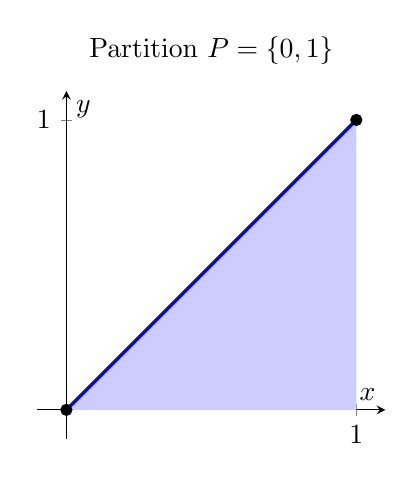
\begin{tikzpicture}
                \begin{axis}[
                axis lines=middle,
                xlabel={$x$},
                ylabel={$y$},
                xmin=-0.1, xmax=1.1,
                ymin=-0.1, ymax=1.1,
                xtick={0,1},
                ytick={0,1},
                width=6cm,
                height=6cm,
                title={Partition $P = \{0, 1\}$}
                ]
                % Shaded area (upper and lower sum coincide for partition P)
                \addplot[fill=blue!20, draw=none, domain=0:1] {x} \closedcycle;
                
                % The function g(x) = x
                \addplot[domain=0:1, samples=2, very thick, blue] {x};
                
                % Mark partition points
                \addplot[only marks, mark=*, mark size=2pt] coordinates {(0,0) (1,1)};
                \end{axis}
            \end{tikzpicture}
            &
            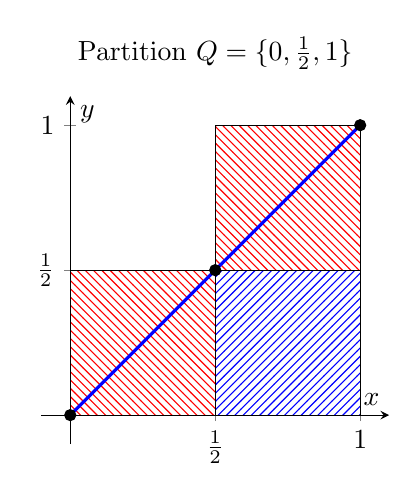
\begin{tikzpicture}
                \begin{axis}[
                axis lines=middle,
                xlabel={$x$},
                ylabel={$y$},
                xmin=-0.1, xmax=1.1,
                ymin=-0.1, ymax=1.1,
                xtick={0,0.5,1},
                ytick={0,0.5,1},
                xticklabels={$0$,$\frac{1}{2}$,$1$},
                yticklabels={$0$,$\frac{1}{2}$,$1$},
                width=6cm,
                height=6cm,
                title={Partition $Q = \{0, \frac{1}{2}, 1\}$}
                ]
                % Lower sum rectangles (northeast lines)
                \addplot[fill=blue!20, pattern=north east lines, pattern color=blue, draw=black] 
                coordinates {(0,0) (0.5,0) (0.5,0) (0,0)} \closedcycle;
                \addplot[fill=blue!20, pattern=north east lines, pattern color=blue, draw=black] 
                coordinates {(0.5,0) (1,0) (1,0.5) (0.5,0.5) (0.5,0)} \closedcycle;
                
                % Upper sum rectangles (northwest lines)
                \addplot[fill=red!20, pattern=north west lines, pattern color=red, draw=black] 
                coordinates {(0,0) (0.5,0) (0.5,0.5) (0,0.5) (0,0)} \closedcycle;
                \addplot[fill=red!20, pattern=north west lines, pattern color=red, draw=black] 
                coordinates {(0.5,0.5) (1,0.5) (1,1) (0.5,1) (0.5,0.5)} \closedcycle;
                
                % The function g(x) = x
                \addplot[domain=0:1, samples=2, very thick, blue] {x};
                
                % Mark partition points
                \addplot[only marks, mark=*, mark size=2pt] coordinates {(0,0) (0.5,0.5) (1,1)};
                \end{axis}
            \end{tikzpicture}
            \end{tabular}
            \end{center}
    \end{proof}

    \item \textit{True or False? Give a proof or a counter-example.}
    
    \rule{1cm}{0.15mm} If $g$ is integrable on $[0,1]$, then so is $g(x^n)$, for all $n \in \mathbb{N}$.
    \begin{proof}[Solution]
    \end{proof}

    \rule{1cm}{0.15mm} If $|f|$ is integrable on $[a,b]$, then so is $f$.
    \begin{proof}[Solution]
    \end{proof}

    \rule{1cm}{0.15mm} If $f$ and $|f|$ are integrable on $[a,b]$, then $|\int_{a}^{b}f| \leq \int_{a}^{b}|f|$.
    \begin{proof}[Solution]
    \end{proof}

\end{enumerate}
\setcounter{chapter}{6}
\chapter{Series, Sequences of Functions, \& Convergence}
\begin{center}
Book References:

Apostol: 8.1 – 8.8, 8.10 – 8.15, 8.17, 8.18, 9.1 – 9.5

Abbott: 6.1 – 6.3
\end{center}

In this section, we will cover:
\begin{itemize}
    \item Infinite Series of Real Numbers
    \item Sequences of Functions
    \item Pointwise and Uniform Convergence
    \item Continuous Limit Theorem
    \item Convergence and Derivatives and Integrals
\end{itemize}

\section{Topic 1}
This is the content for Topic 1.
\begin{thm}{Sample Theorem}
This is a sample theorem in Topic 1.
\end{thm}

\begin{proof}
    Yes.
\end{proof}

This concludes part 7 of Mathematical Analysis.

\end{document}
